Auf Simulink Seite wird die Umgebungssimulation vorgenommen. Dafür müssen die empfangenen Datenpakete auch auf dieser Seite zuerst geparst werden. Anschliessend durchlaufen die Werte einen Algorithmus, welcher neue Werte an das Pixhawk sendet.

\subsubsection{Kommunikation}
Simulink stellt in der 'Instrumental Control Toolbox' TCP/UDP, IP und serielle Kommunikationsblöcke zur Verfügung. Diese Toolbox ist nicht in der HSLU Lizenz einbezogen.\\

\noindent Für die Datenübertragung per Serial Port muss dieser zuerst korrekt konfiguriert werden im Block 'Serial Configuration' (Abbildung \ref{fig:conf_conf}). Die Baud, Kontrollbits, Symbolgrösse, Byte-Reihenfolge sowie ein Timeout müssen angegeben werden.\\

\begin{figure}[H]
  \begin{center}
  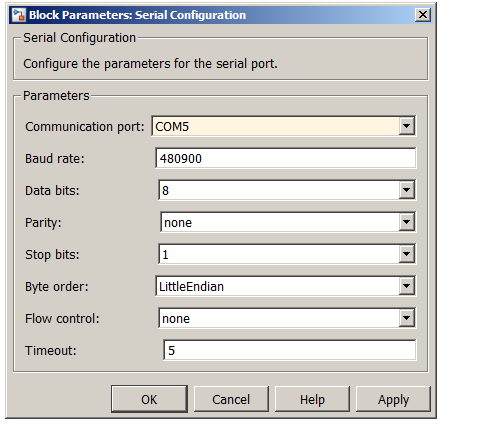
\includegraphics[width=0.5\textwidth]{pic/60_simulink/conf_conf.png}
  \caption{Einstellungen Konfigurationsblock}
  \label{fig:conf_conf}
  \end{center}
\end{figure}


\noindent Der Empfängerblock (Abbildung \ref{fig:conf_rcv}), welcher die Daten ins Simulink einspeist, muss auch konfiguriert werden. Hierbei gilt zu beachten, dass der 'Blocking Mode' ausgeschaltet wird. Dieser Parameter erlaubt, dass die Simulation weiterlaufen kann, obwohl keine neuen Daten empfangen wurden. Der Parser kann auch gleich übergeben werden im Header Feld. In diesem Block wird versucht, alle 50ms ein Packet von 772 Bytes zu empfangen. Diese Paketstruktur entsprechen dem Format von Abbildung \ref{fig:packet1} und muss für die Verwendung zuerst noch geparst werden. Würde man jedes Byte einzeln empfangen, wäre dies sehr ineffizient. Der Block enthält ein Sleep Befehl von 1ms. Dies würde bei einer kurzen Abtastzeit stark ins Gewicht fallen. Bei den 50ms im Projekt ist dies jedoch vernachlässige.\\

\begin{figure}[H]
  \begin{center}
  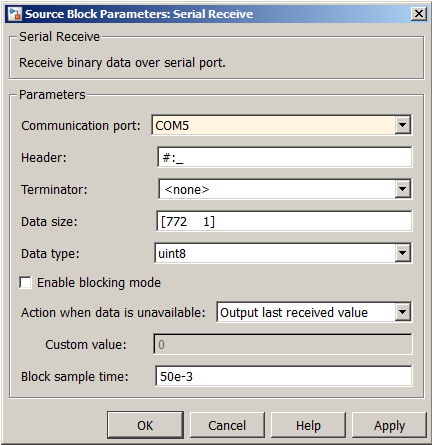
\includegraphics[width=0.5\textwidth]{pic/60_simulink/conf_rcv.png}
  \caption{Einstellungen Empfänger Block}
  \label{fig:conf_rcv}
  \end{center}
\end{figure}

\noindent Der Sendeblock (Abbildung \ref{fig:conf_send}) extrahiert die  Simulationsdaten und sendet diese ans Pixhawk. Die drei Synchronisationsbyte können als Paketkopf übergeben werden.

\noindent
\begin{figure}[H]
  \begin{center}
  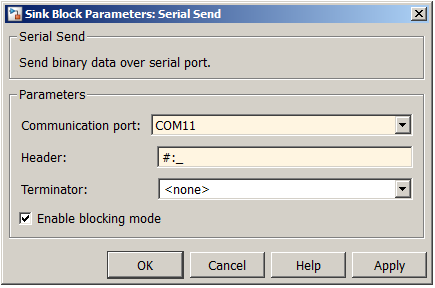
\includegraphics[width=0.5\textwidth]{pic/60_simulink/conf_send.png}
  \caption{Einstellungen Sender Block}
  \label{fig:conf_send}
  \end{center}
\end{figure}

\noindent Diese drei Blöcke übernehmen die gesamte Kommunikation auf Seite Simulink. Der Inhalt des Datenpakets müssen nun gegliedert  und einer Typenumwandlung unterzogen werden.

\clearpage